\documentclass[%
paper=a4,
]
{scrartcl}


\usepackage[english]{babel}
\usepackage[T1]{fontenc}
\usepackage[ansinew]{inputenc}

\usepackage{lmodern} 
\usepackage{microtype}
\usepackage{fixltx2e}

\usepackage{SIunits}

\usepackage[colorlinks = true, citecolor = blue]{hyperref}

\usepackage{graphicx} %%Zum Laden von Grafiken


\title{Sound Event Labeling Tool}
\author{Ivo Trowitzsch}

\begin{document}

\pagestyle{empty} 



\maketitle 				

\section{Motivation}
To effectively train models that identify sound events of particular classes, wav-files containing these sound events need to be annotated by time stamps indicating on- and offsets of these events in the file. A file can contain an arbitrary number of instances of the event class, so it can be arbitrarily many on- and offsets for each file.

Usually such a labeling needs a lot of manual work in a sound editor that enables you to select and listen to arbitrary extracts of the wav file. In addition to the timewise inefficiency because of the tedious selecting of extracts, writing down onset and offset times, etc, working in a sound editor like that also introduces a graphical bias, because the user is misguided to conclude on on- and offsets by the shape of the sound, while this is not necessarily coinciding with the perceptual on- and offsets.

The developed tool shall help to make the process of labeling as fast as possible while maintaining high precision (on- and offsets within 50ms of perceptual "true" on- and offsets) by automatically selecting and presenting extracts of the sound files and letting the user label via a very easy and to-the-task-streamlined user interface, so that he can focus on listening. 


\section{Workflow}
The labeling process of each wav file is divided into subsequent phases:
\begin{enumerate}
\item Pre-labeling to determine which parts of the file should be inspected closer. This can also be skipped.
\begin{itemize}
\item Live-pre-labeling: the user presses a key while he hears the event, useful for long files. (This cannot be used for final event labeling, because it is far too imprecise.)
\item Or energy-based pre-labeling, basically only deselecting parts with no amplitude energy. Useful for isolated events without background.
\end{itemize}
\item A recursive "additive" event finding procedure. The user gets presented blocks of the file (without knowing which part gets played, so without graphical hints) and decides by listening whether the respective block doesn't contain the event class, is a mixture of event and non-event, or is a continous event from beginning to end. In the second case, the block gets divided into two parts and will be presented again. If a block is too small to recognize what is being played back, the block can be increased.
\begin{figure}[h]
	\centering
		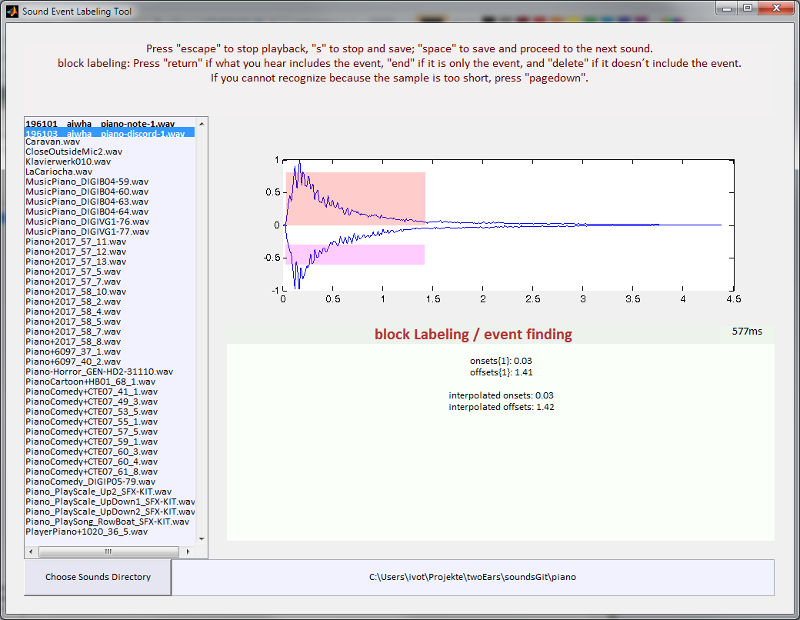
\includegraphics[width=0.80\textwidth]{phase2.png}
	\caption{Phase 2: perceptual event finding}
	\label{fig:phase2}
\end{figure}

\item A "subtractive" event border refining procedure. The user gets presented small blocks at the \emph{border} of the before found events, decreasing its size until the user perceives the event.
\item After this is finished, the user can select ranges in the graphical picture of the sound file to be presented and modified again in the same manner as before. This stage helps to correct for "mistakes".
\begin{figure}[h]
	\centering
  	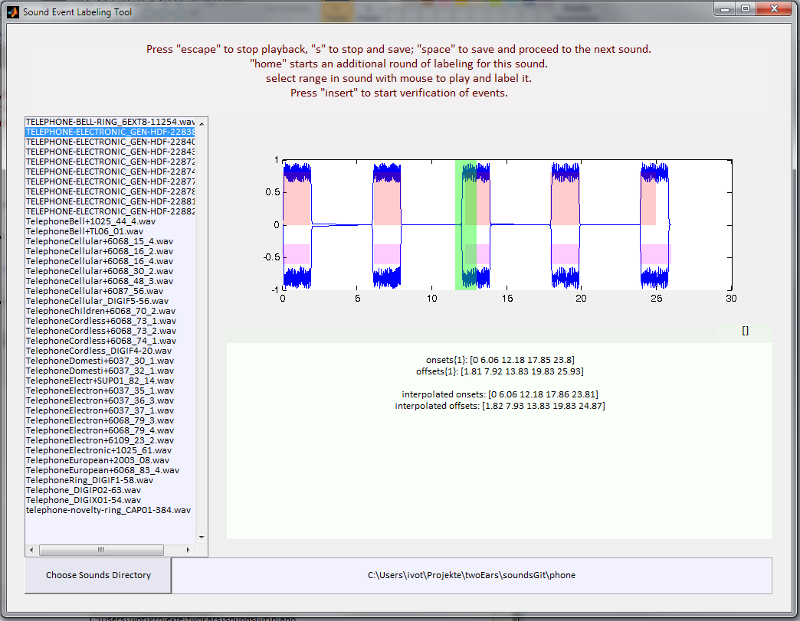
\includegraphics[width=0.8\textwidth]{phase5.png}
	\caption{Phase 4: selecting ranges for relabeling}
	\label{fig:phase5}
\end{figure}

\item As a final step, the user has the option to get presented all positive labeled parts of the file, and decide for each whether the labeling is correct.
\end{enumerate}

If necessary, several rounds can be done for each file with the label times being interpolated between those rounds.

\section{Labeling Result}
The result of the labeling is a text file containing the on- and offset times of the instances of the event in this file, like the following phone event example labeling viewable in figure \ref{fig:phase5} above:\\
\begin{tabular}{cc}
 & \\
0.002268	& 1.814059 \\
6.061224 &	7.922902 \\
12.176871 &	13.827664 \\
17.854875	& 19.825397 \\
23.804989	& 25.927438 \\
 & \\
\end{tabular}

These text files can of course also be loaded into the tool as prelabeling, if already available.


\end{document}
